\documentclass[12pt]{article}
\usepackage{amsmath}
\usepackage{amssymb}
\usepackage{graphicx}
\usepackage{framed}

%\voffset = -5pt
\topmargin = 1pt
\headsep = 5pt
\footskip = 10pt
\textheight = 692pt
\begin{document}

\section{Winston Examples}
\begin{framed}
\begin{verbatim}
using Winston

x = linspace(0, 3pi, 100)
c = cos(x)
s = sin(x)

p = FramedPlot(
        title="title!",
        xlabel="\\Sigma x^2_i",
        ylabel="\\Theta_i")

add(p, FillBetween(x, c, x, s))
add(p, Curve(x, c, color="red"))
add(p, Curve(x, s, color="blue"))

file(p, "example1.png")
\end{verbatim}
\end{framed}
\begin{figure}[h!]
\centering
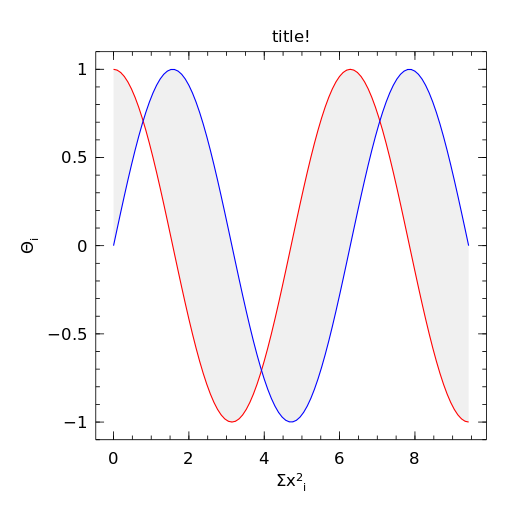
\includegraphics[width=0.8\linewidth]{C:/Users/Computer5/Dropbox/Public/MATLABOctaveJulia/Julia-Winston-Example1}
\caption{Example 1}
\label{fig:Julia-Winston-Example1}
\end{figure}
\newpage
%----------------------------------------------- %
\begin{framed}
\begin{verbatim}
using Winston
srand(42)

p = FramedPlot(
        aspect_ratio=1,
        xrange=(0,100),
        yrange=(0,100))

n = 21
x = linspace(0, 100, n)
yA = 40 + 10randn(n)
yB = x + 5randn(n)

a = Points(x, yA, kind="circle")
setattr(a, label="a points")

b = Points(x, yB)
setattr(b, label="b points")
style(b, kind="filled circle")

s = Slope(1, (0,0), kind="dotted")
setattr(s, label="slope")

l = Legend(.1, .9, {a,b,s})

add(p, s, a, b, l)

file(p, "example2.png")
\end{verbatim}
\end{framed}
\begin{figure}[h!]
\centering
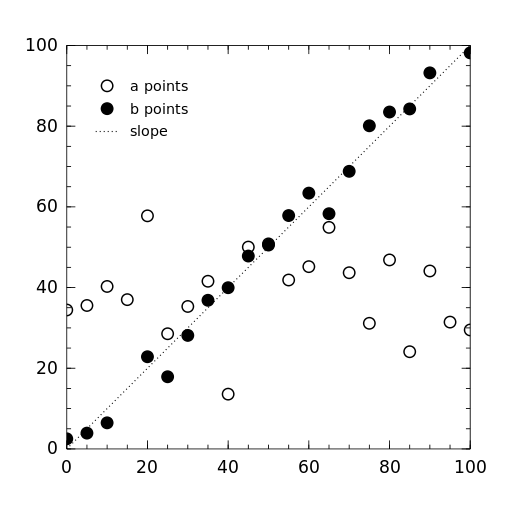
\includegraphics[width=0.6\linewidth]{C:/Users/Computer5/Dropbox/Public/MATLABOctaveJulia/Julia-Winston-Example2}
\caption{Example 2}
\label{fig:Julia-Winston-Example2}
\end{figure}

\newpage
\begin{figure}[h!]
\centering
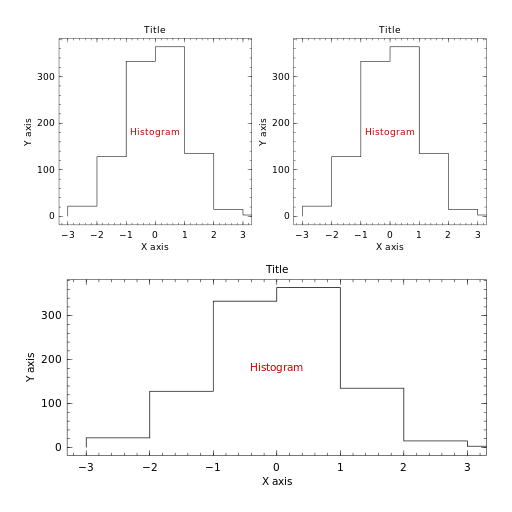
\includegraphics[width=0.9\linewidth]{C:/Users/Computer5/Dropbox/Public/MATLABOctaveJulia/Julia-Winston-Example3}
\caption{Example 3}
\label{fig:Julia-Winston-Example3}
\end{figure}
\newpage

\begin{framed}
\begin{verbatim}
using Winston

x = linspace(0., 2pi, 40)
s = sin(x)
c = cos(x)

inset = FramedPlot(title="inset")
setattr(inset.frame, draw_ticks=false)

add(inset, Curve(x, s, kind="dashed"))

p = FramedPlot(aspect_ratio=1)
setattr(p.frame, tickdir=+1, draw_spine=false)

add(p, SymmetricErrorBarsY(x, s, 0.2*ones(length(x))))
add(p, Points(x, s, color="red"))
add(p, PlotInset((.6,.6), (.95,.95), inset))

file(p, "example4.png")
\end{verbatim}
\end{framed}
%------------------------------------- %

\begin{framed}
\begin{verbatim}
using Winston

x = linspace(0., 2pi, 30)
y = sin(x)

p = FramedArray(2, 2,
        title="title",
        aspect_ratio=0.75,
        xlabel="x label",
        ylabel="y label",
        uniform_limits=true,
        cellspacing=1.)

add(p, LineY(0, kind="dot"))

add(p[1,1], Curve(x, .25*y))
add(p[1,2], Curve(x, .50*y))
add(p[2,1], Curve(x, .75*y))
add(p[2,2], Curve(x, y))

file(p, "example5.png")

\end{verbatim}
\end{framed}
\newpage
\begin{figure}[h!]
\centering
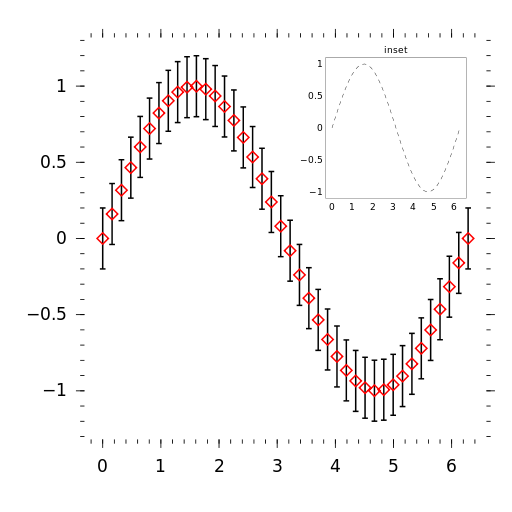
\includegraphics[width=0.9\linewidth]{C:/Users/Computer5/Dropbox/Public/MATLABOctaveJulia/Julia-Winston-Example4}
\caption{Example 4}
\label{fig:Julia-Winston-Example4}
\end{figure}

\newpage
\begin{figure}[h!]
\centering
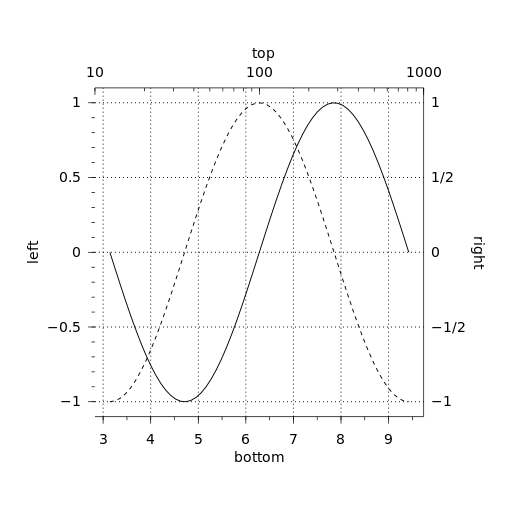
\includegraphics[width=0.9\linewidth]{C:/Users/Computer5/Dropbox/Public/MATLABOctaveJulia/Julia-Winston-Example6}
\caption{Example 6}
\label{fig:Julia-Winston-Example6}
\end{figure}

\begin{figure}[h!]
\centering
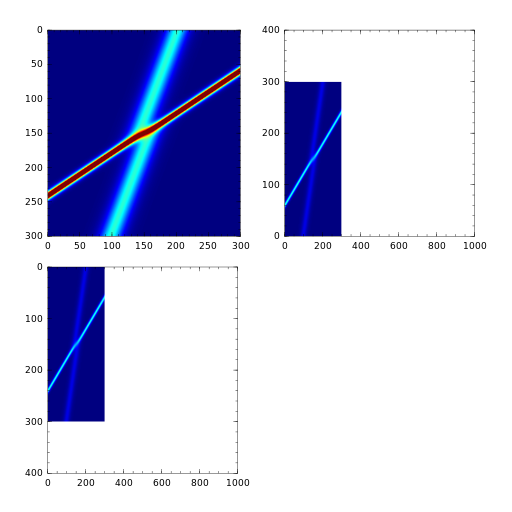
\includegraphics[width=0.9\linewidth]{C:/Users/Computer5/Dropbox/Public/MATLABOctaveJulia/Julia-Winston-Example7}
\caption{Example 7}
\label{fig:Julia-Winston-Example7}
\end{figure}

\end{document}